\documentclass{standalone}
\usepackage{tikz}
\usetikzlibrary{patterns}
\usetikzlibrary{positioning}
\usetikzlibrary{patterns, positioning}
\usetikzlibrary{shapes.misc}
\usepackage[outline]{contour}
\contourlength{1.5pt} 
\usetikzlibrary{calc}
        \usepackage{relsize}
        \tikzset{fontscale/.style = {font=\relsize{#1}}}

\begin{document}
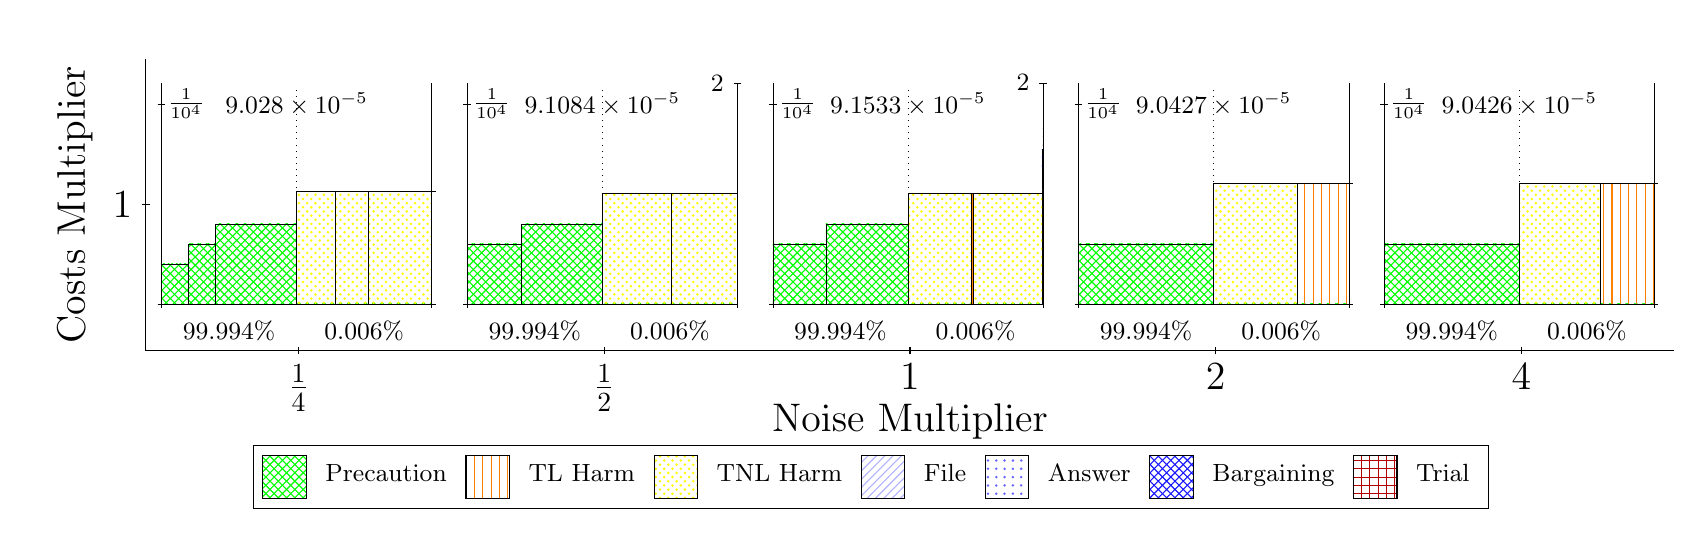
\begin{tikzpicture}
\clip(-0.5,-1.1) rectangle +(20.91,6.2);
\draw[black] (1,1) -- (1,4.7);
\node[rotate=90, fontscale=2, anchor=center] at (0.1, 2.85) {Costs Multiplier};
\draw[black] (0.95,2.85) -- (1.05,2.85);
\node[fontscale=2, anchor=east] at (0.95, 2.85) {1};

\draw[black] (1,1) -- (20.41,1);
\node[fontscale=2, anchor=center] at (10.705, 0.1) {Noise Multiplier};
\draw[black] (2.941,0.95) -- (2.941,1.05);
\node[fontscale=2, anchor=north] at (2.941, 0.95) {$\frac{1}{4}$};
\draw[black] (6.823,0.95) -- (6.823,1.05);
\node[fontscale=2, anchor=north] at (6.823, 0.95) {$\frac{1}{2}$};
\draw[black] (10.705,0.95) -- (10.705,1.05);
\node[fontscale=2, anchor=north] at (10.705, 0.95) {1};
\draw[black] (14.587,0.95) -- (14.587,1.05);
\node[fontscale=2, anchor=north] at (14.587, 0.95) {2};
\draw[black] (18.469,0.95) -- (18.469,1.05);
\node[fontscale=2, anchor=north] at (18.469, 0.95) {4};


\draw[pattern=crosshatch, pattern color=green,draw=black,very thin] (1.2,1.592) rectangle (1.543,2.1);
\draw[pattern=crosshatch, pattern color=green,draw=black,very thin] (1.543,1.592) rectangle (1.8864,2.354);
\draw[pattern=crosshatch, pattern color=green,draw=black,very thin] (1.8864,1.592) rectangle (2.916,2.608);
\draw[pattern=crosshatch, pattern color=green,draw=black,very thin] (2.916,1.592) rectangle (3.4103,1.592);
\draw[pattern=crosshatch dots, pattern color=yellow,draw=black,very thin] (2.916,1.592) rectangle (3.4103,3.0216);
\draw[pattern=crosshatch, pattern color=green,draw=black,very thin] (3.4103,1.592) rectangle (3.822,1.592);
\draw[pattern=crosshatch dots, pattern color=yellow,draw=black,very thin] (3.4103,1.592) rectangle (3.822,3.0216);
\draw[pattern=crosshatch, pattern color=green,draw=black,very thin] (3.822,1.592) rectangle (4.6318,1.5921);
\draw[pattern=crosshatch dots, pattern color=yellow,draw=black,very thin] (3.822,1.5921) rectangle (4.6318,3.0216);
\draw[pattern=crosshatch, pattern color=green,draw=black,very thin] (4.6318,1.592) rectangle (4.632,1.592);
\draw[pattern=crosshatch dots, pattern color=yellow,draw=black,very thin] (4.6318,1.592) rectangle (4.632,3.0216);
\draw[pattern=north east lines, pattern color=blue!30,draw=black,very thin] (4.6318,3.0216) rectangle (4.632,3.1645);
\draw[pattern=dots,  pattern color=blue!60,draw=black,very thin] (4.6318,3.1645) rectangle (4.632,3.3075);
\draw[pattern=crosshatch,      pattern color=blue!90,draw=black,very thin] (4.6318,3.3075) rectangle (4.632,3.5934);
\node[font=\small,text=black,anchor=north] at (2.916, 4.4) {$9.028\times 10^{-5}$};
\draw[black,very thin] (1.2,1.592) -- (1.2,4.4);
\draw[black,very thin] (1.15,1.592) -- (1.25,1.592);
\node[font=\small,text=black, anchor=west] at (1.15, 1.592) {};
\draw[black,very thin] (1.15,4.1321) -- (1.25,4.1321);
\node[font=\small,text=black, anchor=west] at (1.15, 4.1321) {$\frac{1}{10^{4}}$};

\draw[black,dotted,very thin] (2.916,1.6762) -- (2.916,4.3158);
\draw[black,very thin] (4.632,1.592) -- (4.632,4.4);
\draw[black,very thin] (4.582,1.592) -- (4.682,1.592);
\node[font=\small,text=black, anchor=east] at (4.582, 1.592) {\contour{white}{}};
\draw[black,very thin] (4.582,3.0215) -- (4.682,3.0215);
\node[font=\small,text=black, anchor=east] at (4.582, 3.0215) {\contour{white}{}};

\draw[black,very thin] (1.2,1.592) -- (4.632,1.592);
\draw[black,very thin] (1.2,1.542) -- (1.2,1.642);
\node[font=\small,text=black, anchor=north] at (1.2, 1.542) {};
\draw[black,very thin] (4.632,1.542) -- (4.632,1.642);
\node[font=\small,text=black, anchor=north] at (4.632, 1.542) {};

\node[font=\small,text=black,anchor=south] at (2.058, 0.992) {99.994\%};
\node[font=\small,text=black,anchor=south] at (3.774, 0.992) {0.006\%};

\draw[pattern=crosshatch, pattern color=green,draw=black,very thin] (5.082,1.592) rectangle (5.7682,2.354);
\draw[pattern=crosshatch, pattern color=green,draw=black,very thin] (5.7682,1.592) rectangle (6.798,2.608);
\draw[pattern=crosshatch, pattern color=green,draw=black,very thin] (6.798,1.592) rectangle (7.6786,1.592);
\draw[pattern=crosshatch dots, pattern color=yellow,draw=black,very thin] (6.798,1.592) rectangle (7.6786,2.9913);
\draw[pattern=crosshatch, pattern color=green,draw=black,very thin] (7.6786,1.592) rectangle (8.514,1.5921);
\draw[pattern=crosshatch dots, pattern color=yellow,draw=black,very thin] (7.6786,1.5921) rectangle (8.514,2.9913);
\node[font=\small,text=black,anchor=north] at (6.798, 4.4) {$9.1084\times 10^{-5}$};
\draw[black,very thin] (5.082,1.592) -- (5.082,4.4);
\draw[black,very thin] (5.032,1.592) -- (5.132,1.592);
\node[font=\small,text=black, anchor=west] at (5.032, 1.592) {};
\draw[black,very thin] (5.032,4.1321) -- (5.132,4.1321);
\node[font=\small,text=black, anchor=west] at (5.032, 4.1321) {$\frac{1}{10^{4}}$};

\draw[black,dotted,very thin] (6.798,1.6762) -- (6.798,4.3158);
\draw[black,very thin] (8.514,1.592) -- (8.514,4.4);
\draw[black,very thin] (8.464,4.3904) -- (8.564,4.3904);
\node[font=\small,text=black, anchor=east] at (8.464, 4.3904) {\contour{white}{2}};

\draw[black,very thin] (5.082,1.592) -- (8.514,1.592);
\draw[black,very thin] (5.082,1.542) -- (5.082,1.642);
\node[font=\small,text=black, anchor=north] at (5.082, 1.542) {};
\draw[black,very thin] (8.514,1.542) -- (8.514,1.642);
\node[font=\small,text=black, anchor=north] at (8.514, 1.542) {};

\node[font=\small,text=black,anchor=south] at (5.94, 0.992) {99.994\%};
\node[font=\small,text=black,anchor=south] at (7.656, 0.992) {0.006\%};

\draw[pattern=crosshatch, pattern color=green,draw=black,very thin] (8.964,1.592) rectangle (9.6365,2.354);
\draw[pattern=crosshatch, pattern color=green,draw=black,very thin] (9.6365,1.592) rectangle (10.68,2.608);
\draw[pattern=crosshatch, pattern color=green,draw=black,very thin] (10.68,1.592) rectangle (10.682,1.592);
\draw[pattern=north east lines, pattern color=blue!30,draw=black,very thin] (10.68,1.592) rectangle (10.682,1.7324);
\draw[pattern=dots,  pattern color=blue!60,draw=black,very thin] (10.68,1.7324) rectangle (10.682,1.8728);
\draw[pattern=crosshatch,      pattern color=blue!90,draw=black,very thin] (10.68,1.8728) rectangle (10.682,2.1536);
\draw[pattern=crosshatch, pattern color=green,draw=black,very thin] (10.682,1.592) rectangle (11.489,1.592);
\draw[pattern=crosshatch dots, pattern color=yellow,draw=black,very thin] (10.682,1.592) rectangle (11.489,2.996);
\draw[pattern=crosshatch, pattern color=green,draw=black,very thin] (11.489,1.592) rectangle (11.508,1.592);
\draw[pattern=vertical lines, pattern color=orange,draw=black,very thin] (11.489,1.592) rectangle (11.508,2.996);
\draw[pattern=crosshatch, pattern color=green,draw=black,very thin] (11.508,1.592) rectangle (12.38,1.5921);
\draw[pattern=crosshatch dots, pattern color=yellow,draw=black,very thin] (11.508,1.5921) rectangle (12.38,2.996);
\draw[pattern=crosshatch, pattern color=green,draw=black,very thin] (12.38,1.592) rectangle (12.386,1.592);
\draw[pattern=crosshatch dots, pattern color=yellow,draw=black,very thin] (12.38,1.592) rectangle (12.386,2.996);
\draw[pattern=north east lines, pattern color=blue!30,draw=black,very thin] (12.38,2.996) rectangle (12.386,3.1364);
\draw[pattern=dots,  pattern color=blue!60,draw=black,very thin] (12.38,3.1364) rectangle (12.386,3.2768);
\draw[pattern=crosshatch,      pattern color=blue!90,draw=black,very thin] (12.38,3.2768) rectangle (12.386,3.5576);
\draw[pattern=crosshatch, pattern color=green,draw=black,very thin] (12.386,1.592) rectangle (12.393,1.592);
\draw[pattern=vertical lines, pattern color=orange,draw=black,very thin] (12.386,1.592) rectangle (12.393,2.996);
\draw[pattern=north east lines, pattern color=blue!30,draw=black,very thin] (12.386,2.996) rectangle (12.393,3.1364);
\draw[pattern=dots,  pattern color=blue!60,draw=black,very thin] (12.386,3.1364) rectangle (12.393,3.2768);
\draw[pattern=crosshatch,      pattern color=blue!90,draw=black,very thin] (12.386,3.2768) rectangle (12.393,3.5576);
\draw[pattern=crosshatch, pattern color=green,draw=black,very thin] (12.393,1.592) rectangle (12.395,1.592);
\draw[pattern=crosshatch dots, pattern color=yellow,draw=black,very thin] (12.393,1.592) rectangle (12.395,2.996);
\draw[pattern=north east lines, pattern color=blue!30,draw=black,very thin] (12.393,2.996) rectangle (12.395,3.1364);
\draw[pattern=dots,  pattern color=blue!60,draw=black,very thin] (12.393,3.1364) rectangle (12.395,3.2768);
\draw[pattern=crosshatch,      pattern color=blue!90,draw=black,very thin] (12.393,3.2768) rectangle (12.395,3.5576);
\draw[pattern=grid,            pattern color=red!70!black,draw=black,very thin] (12.393,3.5576) rectangle (12.395,3.8384);
\draw[pattern=crosshatch, pattern color=green,draw=black,very thin] (12.395,1.592) rectangle (12.396,1.592);
\draw[pattern=vertical lines, pattern color=orange,draw=black,very thin] (12.395,1.592) rectangle (12.396,2.996);
\draw[pattern=north east lines, pattern color=blue!30,draw=black,very thin] (12.395,2.996) rectangle (12.396,3.1364);
\draw[pattern=dots,  pattern color=blue!60,draw=black,very thin] (12.395,3.1364) rectangle (12.396,3.2768);
\draw[pattern=crosshatch,      pattern color=blue!90,draw=black,very thin] (12.395,3.2768) rectangle (12.396,3.5576);
\draw[pattern=grid,            pattern color=red!70!black,draw=black,very thin] (12.395,3.5576) rectangle (12.396,3.8384);
\node[font=\small,text=black,anchor=north] at (10.68, 4.4) {$9.1533\times 10^{-5}$};
\draw[black,very thin] (8.964,1.592) -- (8.964,4.4);
\draw[black,very thin] (8.914,1.592) -- (9.014,1.592);
\node[font=\small,text=black, anchor=west] at (8.914, 1.592) {};
\draw[black,very thin] (8.914,4.1321) -- (9.014,4.1321);
\node[font=\small,text=black, anchor=west] at (8.914, 4.1321) {$\frac{1}{10^{4}}$};

\draw[black,dotted,very thin] (10.68,1.6762) -- (10.68,4.3158);
\draw[black,very thin] (12.396,1.592) -- (12.396,4.4);
\draw[black,very thin] (12.346,4.3999) -- (12.446,4.3999);
\node[font=\small,text=black, anchor=east] at (12.346, 4.3999) {\contour{white}{2}};

\draw[black,very thin] (8.964,1.592) -- (12.396,1.592);
\draw[black,very thin] (8.964,1.542) -- (8.964,1.642);
\node[font=\small,text=black, anchor=north] at (8.964, 1.542) {};
\draw[black,very thin] (12.396,1.542) -- (12.396,1.642);
\node[font=\small,text=black, anchor=north] at (12.396, 1.542) {};

\node[font=\small,text=black,anchor=south] at (9.822, 0.992) {99.994\%};
\node[font=\small,text=black,anchor=south] at (11.538, 0.992) {0.006\%};

\draw[pattern=crosshatch, pattern color=green,draw=black,very thin] (12.846,1.592) rectangle (14.562,2.354);
\draw[pattern=crosshatch, pattern color=green,draw=black,very thin] (14.562,1.592) rectangle (15.621,1.592);
\draw[pattern=crosshatch dots, pattern color=yellow,draw=black,very thin] (14.562,1.592) rectangle (15.621,3.127);
\draw[pattern=crosshatch, pattern color=green,draw=black,very thin] (15.621,1.592) rectangle (16.278,1.592);
\draw[pattern=vertical lines, pattern color=orange,draw=black,very thin] (15.621,1.592) rectangle (16.278,3.127);
\node[font=\small,text=black,anchor=north] at (14.562, 4.4) {$9.0427\times 10^{-5}$};
\draw[black,very thin] (12.846,1.592) -- (12.846,4.4);
\draw[black,very thin] (12.796,1.592) -- (12.896,1.592);
\node[font=\small,text=black, anchor=west] at (12.796, 1.592) {};
\draw[black,very thin] (12.796,4.1321) -- (12.896,4.1321);
\node[font=\small,text=black, anchor=west] at (12.796, 4.1321) {$\frac{1}{10^{4}}$};

\draw[black,dotted,very thin] (14.562,1.6762) -- (14.562,4.3158);
\draw[black,very thin] (16.278,1.592) -- (16.278,4.4);
\draw[black,very thin] (16.228,1.592) -- (16.328,1.592);
\node[font=\small,text=black, anchor=east] at (16.228, 1.592) {\contour{white}{}};
\draw[black,very thin] (16.228,3.127) -- (16.328,3.127);
\node[font=\small,text=black, anchor=east] at (16.228, 3.127) {\contour{white}{}};

\draw[black,very thin] (12.846,1.592) -- (16.278,1.592);
\draw[black,very thin] (12.846,1.542) -- (12.846,1.642);
\node[font=\small,text=black, anchor=north] at (12.846, 1.542) {};
\draw[black,very thin] (16.278,1.542) -- (16.278,1.642);
\node[font=\small,text=black, anchor=north] at (16.278, 1.542) {};

\node[font=\small,text=black,anchor=south] at (13.704, 0.992) {99.994\%};
\node[font=\small,text=black,anchor=south] at (15.42, 0.992) {0.006\%};

\draw[pattern=crosshatch, pattern color=green,draw=black,very thin] (16.728,1.592) rectangle (18.444,2.354);
\draw[pattern=crosshatch, pattern color=green,draw=black,very thin] (18.444,1.592) rectangle (19.477,1.592);
\draw[pattern=crosshatch dots, pattern color=yellow,draw=black,very thin] (18.444,1.592) rectangle (19.477,3.127);
\draw[pattern=crosshatch, pattern color=green,draw=black,very thin] (19.477,1.592) rectangle (20.16,1.592);
\draw[pattern=vertical lines, pattern color=orange,draw=black,very thin] (19.477,1.592) rectangle (20.16,3.127);
\node[font=\small,text=black,anchor=north] at (18.444, 4.4) {$9.0426\times 10^{-5}$};
\draw[black,very thin] (16.728,1.592) -- (16.728,4.4);
\draw[black,very thin] (16.678,1.592) -- (16.778,1.592);
\node[font=\small,text=black, anchor=west] at (16.678, 1.592) {};
\draw[black,very thin] (16.678,4.1321) -- (16.778,4.1321);
\node[font=\small,text=black, anchor=west] at (16.678, 4.1321) {$\frac{1}{10^{4}}$};

\draw[black,dotted,very thin] (18.444,1.6762) -- (18.444,4.3158);
\draw[black,very thin] (20.16,1.592) -- (20.16,4.4);
\draw[black,very thin] (20.11,1.592) -- (20.21,1.592);
\node[font=\small,text=black, anchor=east] at (20.11, 1.592) {\contour{white}{}};
\draw[black,very thin] (20.11,3.1269) -- (20.21,3.1269);
\node[font=\small,text=black, anchor=east] at (20.11, 3.1269) {\contour{white}{}};

\draw[black,very thin] (16.728,1.592) -- (20.16,1.592);
\draw[black,very thin] (16.728,1.542) -- (16.728,1.642);
\node[font=\small,text=black, anchor=north] at (16.728, 1.542) {};
\draw[black,very thin] (20.16,1.542) -- (20.16,1.642);
\node[font=\small,text=black, anchor=north] at (20.16, 1.542) {};

\node[font=\small,text=black,anchor=south] at (17.586, 0.992) {99.994\%};
\node[font=\small,text=black,anchor=south] at (19.302, 0.992) {0.006\%};

\coordinate (LegendAnchor) at (10.205000000000002,0);
\begin{scope}[align=center]
\matrix[scale=0.6,draw=black,below=0.2cm of LegendAnchor,nodes={draw},column sep=0.12cm]{
\node[rectangle,draw,minimum width=0.55cm,minimum height=0.55cm,pattern=crosshatch, pattern color=green]{}; &
        \node[draw=none,font=\small]{Precaution}; &
\node[rectangle,draw,minimum width=0.55cm,minimum height=0.55cm,pattern=vertical lines, pattern color=orange]{}; &
        \node[draw=none,font=\small]{TL Harm}; &
\node[rectangle,draw,minimum width=0.55cm,minimum height=0.55cm,pattern=crosshatch dots, pattern color=yellow]{}; &
        \node[draw=none,font=\small]{TNL Harm}; &
\node[rectangle,draw,minimum width=0.55cm,minimum height=0.55cm,pattern=north east lines, pattern color=blue!30]{}; &
        \node[draw=none,font=\small]{File}; &
\node[rectangle,draw,minimum width=0.55cm,minimum height=0.55cm,pattern=dots, pattern color=blue!60]{}; &
        \node[draw=none,font=\small]{Answer}; &
\node[rectangle,draw,minimum width=0.55cm,minimum height=0.55cm,pattern=crosshatch, pattern color=blue!90]{}; &
        \node[draw=none,font=\small]{Bargaining}; &
\node[rectangle,draw,minimum width=0.55cm,minimum height=0.55cm,pattern=grid, pattern color=red!70!black]{}; &
        \node[draw=none,font=\small]{Trial}; \\
};\end{scope}

\end{tikzpicture}
\end{document}